\documentclass[pdf,oneside]{oucthesis}
% pdf: 便于阅读的电子版,去除掉多余的空白页,加入超链接等
% print:打印版本,添加空白页,便于双面打印,禁用超链接



% ========================================
%|             论文信息填写               |
% ========================================
\title{北大西洋亚极地区域多尺度海洋过程能量交换}


% ========================================
%                包引用                 
% ========================================
\usepackage{booktabs}
\usepackage{multirow}
\usepackage{setspace}
\usepackage{amsthm}
\usepackage{algorithm}
\usepackage{algorithmicx}
\usepackage{algpseudocode}
\usepackage{caption}
\captionsetup{font={small}}

% 内容区域
\begin{document}

% 封面
% 学位论文封面页
\begin{titlepage}

\noindent\textbf{\zihao{4}{分类号:} \hspace*{210pt} {学校代码:10423} \\ {UDC:} \hspace*{216pt} {学 ~~~ 号:}}
\vskip50pt
\par \vskip20pt

% 中文标题
\begin{spacing}{1.5}
\centering{\fontsize{20pt}{30pt}\selectfont\heiti 北大西洋亚极地区域多尺度海洋过程能量交换}
\par \vskip30pt

% 英文标题
\centering{\fontsize{20pt}{80pt}\selectfont\textbf{Energy Exchange among Multi-scale Processes in the Subpolar North Atlantic}}
\end{spacing}

% 居中,左侧两端对齐,列宽与研究生院范例相同,3.19cm
\par\vskip110pt
\begin{center}
    \begin{tabular}{l l}  % 左对齐两列
        \makebox[3.19cm][s]{\fontsize{14pt}{21pt}\selectfont\heiti 作\hspace{\fill}者}:
        & \fontsize{14pt}{21pt}\selectfont 某某某 \\
        \makebox[3.19cm][s]{\fontsize{14pt}{21pt}\selectfont\heiti 指\hspace{\fill}导\hspace{\fill}教\hspace{\fill}师}:
        & \fontsize{14pt}{21pt}\selectfont 某某某 ~ 教授 \\
        \makebox[3.19cm][s]{\fontsize{14pt}{21pt}\selectfont\heiti 学\hspace{\fill}位\hspace{\fill}类\hspace{\fill}型}:
        & \fontsize{14pt}{21pt}\selectfont 学术学位 \\
        \makebox[3.19cm][s]{\fontsize{14pt}{21pt}\selectfont\heiti 专\hspace{\fill}业\hspace{\fill}名\hspace{\fill}称}:
        & \fontsize{14pt}{21pt}\selectfont 计算机科学与技术 \\
        \makebox[3.19cm][s]{\fontsize{14pt}{21pt}\selectfont\heiti 研\hspace{\fill}究\hspace{\fill}方\hspace{\fill}向}:
        & \fontsize{14pt}{21pt}\selectfont 计算机软件与理论 \\
        \makebox[3.19cm][s]{\fontsize{14pt}{21pt}\selectfont\heiti 授予学位单位}:
        & \fontsize{14pt}{21pt}\selectfont 中国海洋大学 \\
    \end{tabular}
\end{center}

\par\vskip80pt
\centering{\fontsize{14}{32}\selectfont\heiti 日期:\today}

\end{titlepage}

% 学位论文答辩委员会
% 学位论文答辩委员会页
\begin{titlepage}

\par \vskip10pt
\centering{\fontsize{16pt}{24pt}\selectfont\heiti 学位论文答辩委员会}
\par \vskip50pt


\begin{table}[htbp]
\centering
\renewcommand\arraystretch{1.8}
\begin{tabular}{|c|c|c|c|c|}
\hline
答辩时间 & \multicolumn{4}{c|}{ ~~~ 年 ~~~ 月 ~~~ 日} \\ \hline
答辩地点 & \multicolumn{4}{c|}{}\\ \hline
\multicolumn{5}{|c|}{答辩委员会组成}\\ \hline
~~~ 组成 ~~~ & ~~~ 姓名 ~~~ & ~~~ 专业技术职务 ~~~ & ~~~ 工作单位 ~~~ & ~~~~~ 签名 ~~~~~ \\ \hline
主席 & & & & \\ \hline
\multirow{6}{*}{委员} & & & & \\ \cline{2-5}
 & & & & \\ \cline{2-5}
 & & & & \\ \cline{2-5}
 & & & & \\ \cline{2-5}
 & & & & \\ \cline{2-5}
 & & & & \\ \hline
\end{tabular}
\end{table}

    
\end{titlepage}

% 独创性声明
% 学位论文独创声明
\begin{titlepage}

\par\vskip30pt
\begin{spacing}{1.5}
\centering{\fontsize{16pt}{24pt}\selectfont\heiti 学位论文独创声明}
\end{spacing}

\par\vskip20pt
本人所呈交的学位论文是本人在导师指导下进行的研究工作及取得的研究成果。除了文中加以标注和致谢的地方外,论文中不包含其他人已经发表或撰写过的研究成果,也不包含为获得\underline{~~~~~~~~~~~~~~~~~~~~~~~~~~~~~~~(注:如没有其他需要特别声明的,本栏可空)}或其他教育机构的学位或证书使用过的材料。对本文的研究作出重要贡献的个人和集体,均已在文中以明确方式标明。本声明的法律责任由本人承担。

\par\vskip60pt

学位论文作者签名:\hspace*{160pt} 日期:\today

\begin{spacing}{1.5}
\centering{- - - - - - - - - - - - - - - - - - - - - - - - - - - - - - - - - - - - - - - - - - - - - - - - - - - - - - - - - }
\end{spacing}

\begin{spacing}{1.5}
\centering{\fontsize{16pt}{24pt}\selectfont\heiti 学位论文版权使用授权书}
\end{spacing}

\par\vskip20pt
本学位论文作者完全了解国家有关保留、使用学位论文的法律、法规和学校有关规定,并同意以下事项:

1.学校有权保留并向国家有关部门或机构送交本学位论文的复印件和电子版,允许论文被查阅和借阅;

2.学校可以将本学位论文的全部或部分内容编入有关数据库进行检索,可以采用影印、缩印或扫描等复制手段保存、汇编本学位论文;

3.学校可以基于教学及科研需要合理使用本学位论文。

需保密的学位论文在解密后适用本授权书。

\par\vskip60pt
学位论文作者签名:\hspace*{160pt} 导师签名:
\par\vskip20pt
日期:\today \hspace*{135pt} 日期:\today

\end{titlepage}

% 从摘要开始,设置行距为20磅
\setlength{\baselineskip}{20pt}

% 中文摘要
% 中文摘要
\pagenumbering{1}
\begin{abstract}

海洋中尺度涡旋是海洋中动能串级的重要枢纽,占据海洋70\%以上的海洋动能。关于中尺度涡旋动能来源与耗散问题,是影响海洋动力学平衡的重要问题。目前研究认为,中尺度涡旋能够与亚中尺度过程和海洋近惯性内波相互作用,是解决中尺度涡旋动能来源与耗散的潜在渠道。目前对于三者之间相互作用研究多集中于中纬度地区和南大洋,尚缺乏对北大西洋亚极地海区的系统研究。

北大西洋亚极地区域由于强烈的混合层深度变化和风暴,存在丰富的中尺度、亚中尺度过程和近惯性内波,这些过程之间有着复杂的相互作用关系,能够调节上层海洋混合、再层化以及深层对流等过程。因此,对北大西洋中尺度涡旋、亚中尺度过程以及海洋内波之间能量交换过程的研究是十分必要的,有助于提高。

海洋中尺度涡旋是海洋中动能串级的重要枢纽,占据海洋70\%以上的海洋动能。关于中尺度涡旋动能来源与耗散问题,是影响海洋动力学平衡的重要问题。目前研究认为,中尺度涡旋能够与亚中尺度过程和海洋近惯性内波相互作用,是解决中尺度涡旋动能来源与耗散的潜在渠道。目前对于三者之间相互作用研究多集中于中纬度地区和南大洋,尚缺乏对北大西洋亚极地海区的系统研究。

北大西洋亚极地区域由于强烈的混合层深度变化和风暴,存在丰富的中尺度、亚中尺度过程和近惯性内波,这些过程之间有着复杂的相互作用关系,能够调节上层海洋混合、再层化以及深层对流等过程。因此,对北大西洋中尺度涡旋、亚中尺度过程以及海洋内波之间能量交换过程的研究是十分必要的,有助于提高。

海洋中尺度涡旋是海洋中动能串级的重要枢纽,占据海洋70\%以上的海洋动能。关于中尺度涡旋动能来源与耗散问题,是影响海洋动力学平衡的重要问题。目前研究认为,中尺度涡旋能够与亚中尺度过程和海洋近惯性内波相互作用,是解决中尺度涡旋动能来源与耗散的潜在渠道。目前对于三者之间相互作用研究多集中于中纬度地区和南大洋,尚缺乏对北大西洋亚极地海区的系统研究。

北大西洋亚极地区域由于强烈的混合层深度变化和风暴,存在丰富的中尺度、亚中尺度过程和近惯性内波,这些过程之间有着复杂的相互作用关系,能够调节上层海洋混合、再层化以及深层对流等过程。因此,对北大西洋中尺度涡旋、亚中尺度过程以及海洋内波之间能量交换过程的研究是十分必要的,有助于提高。

海洋中尺度涡旋是海洋中动能串级的重要枢纽,占据海洋70\%以上的海洋动能。关于中尺度涡旋动能来源与耗散问题,是影响海洋动力学平衡的重要问题。目前研究认为,中尺度涡旋能够与亚中尺度过程和海洋近惯性内波相互作用,是解决中尺度涡旋动能来源与耗散的潜在渠道。目前对于三者之间相互作用研究多集中于中纬度地区和南大洋,尚缺乏对北大西洋亚极地海区的系统研究。

北大西洋亚极地区域由于强烈的混合层深度变化和风暴,存在丰富的中尺度、亚中尺度过程和近惯性内波,这些过程之间有着复杂的相互作用关系,能够调节上层海洋混合、再层化以及深层对流等过程。因此,对北大西洋中尺度涡旋、亚中尺度过程以及海洋内波之间能量交换过程的研究是十分必要的,有助于提高。

\noindent\textbf{关键词:}北大西洋亚极地区域;中尺度;亚中尺度

\end{abstract}

% 英文摘要
\begin{enabstract}

Mesoscale eddies in the ocean are an important hub of energy cascade, accounting for over 70\% of the oceanic kinetic energy. The issue of the energy source and dissipation of mesoscale eddies is a significant problem that affects the balance of ocean dynamics. Current studies suggest that mesoscale eddies can interact with submesoscale processes and near-inertial internal waves, providing a potential channel to address the energy source and dissipation of mesoscale eddies. However, research on the interactions among the three is mostly concentrated in mid-latitudes and the Southern Ocean, and there is a lack of systematic study on the subpolar North Atlantic region.

The subpolar North Atlantic region, with its strong variations in the depth of the mixed layer and storms, has rich mesoscale and submesoscale processes and near-inertial internal waves. These processes have complex interactions that can regulate upper ocean mixing, restratification, and deep convection. Therefore, it is essential to study the energy exchange processes among mesoscale eddies, submesoscale processes, and internal waves in the North Atlantic region to improve.

Mesoscale eddies in the ocean are an important hub of energy cascade, accounting for over 70\% of the oceanic kinetic energy. The issue of the energy source and dissipation of mesoscale eddies is a significant problem that affects the balance of ocean dynamics. Current studies suggest that mesoscale eddies can interact with submesoscale processes and near-inertial internal waves, providing a potential channel to address the energy source and dissipation of mesoscale eddies. However, research on the interactions among the three is mostly concentrated in mid-latitudes and the Southern Ocean, and there is a lack of systematic study on the subpolar North Atlantic region.

The subpolar North Atlantic region, with its strong variations in the depth of the mixed layer and storms, has rich mesoscale and submesoscale processes and near-inertial internal waves. These processes have complex interactions that can regulate upper ocean mixing, restratification, and deep convection. Therefore, it is essential to study the energy exchange processes among mesoscale eddies, submesoscale processes, and internal waves in the North Atlantic region to improve.

Mesoscale eddies in the ocean are an important hub of energy cascade, accounting for over 70\% of the oceanic kinetic energy. The issue of the energy source and dissipation of mesoscale eddies is a significant problem that affects the balance of ocean dynamics. Current studies suggest that mesoscale eddies can interact with submesoscale processes and near-inertial internal waves, providing a potential channel to address the energy source and dissipation of mesoscale eddies. However, research on the interactions among the three is mostly concentrated in mid-latitudes and the Southern Ocean, and there is a lack of systematic study on the subpolar North Atlantic region.

The subpolar North Atlantic region, with its strong variations in the depth of the mixed layer and storms, has rich mesoscale and submesoscale processes and near-inertial internal waves. These processes have complex interactions that can regulate upper ocean mixing, restratification, and deep convection. Therefore, it is essential to study the energy exchange processes among mesoscale eddies, submesoscale processes, and internal waves in the North Atlantic region to improve.

\noindent\textbf{Key Words:} mesoscale; submesoscale

\end{enabstract}






% 目录
\tableofcontents % 中文目录
\tableofengcontents % 英文目录


% 图表目录
\newcommand{\loflabel}{图} 
\renewcommand{\numberline}[1]{\loflabel~#1\hspace*{1em}}
\renewcommand{\listfigurename}{插图清单} 
\begin{center}
\clearpage
\phantomsection\addcontentsline{toc}{chapter}{插图清单}
\phantomsection\addengcontent{chapter}{Figure list}
{\listoffigures}
\end{center}


\newcommand{\lotlabel}{表}
\renewcommand{\numberline}[1]{\lotlabel~#1\hspace*{1em}}
\renewcommand{\listtablename}{表格清单} 
\begin{center}
\clearpage
\phantomsection\addcontentsline{toc}{chapter}{表格清单}
\phantomsection\addengcontent{chapter}{Table list}
{\listoftables}
\end{center}



% 正文
\mainmatter
\pagenumbering{arabic}


\chapter{绪论}
\enchapter{Introduction}


\section{北大西洋海洋多尺度能量串级的研究意义}
\ensection{Significance of multi-scale energy cascade in the North Atlantic Ocean}

海洋中的环流受到地球自转的影响,动能主要集中在海洋的大尺度环流,如黑潮、湾流和中尺度涡旋等空间尺度大于地转尺度的运动上。根据目前已有的卫星高度计数据,中尺度能量占据了大洋总能量的70\%以上。中尺度庞大的动能来源与去向问题一直是本世纪海洋动力学研究的热点问题。Wunsch和Ferrari在2004年回顾性的工作指出 $\cdots\cdots$ 


\section{中尺度涡旋与亚中尺度过程之间的能量串级}
\ensection{Energy cascade between mesoscale eddies and sub-mesoscale processes}

\subsection{中尺度漩涡}
\ensubsection{Mesoscale eddy}

中尺度涡旋在海洋中广泛存在,其空间尺度通常在50公里-500公里,被认为是低阶近似满足地转平衡的最小尺度海洋运动过程,因此其水平运动远远大于垂直运动,具有较小罗斯贝数和较大理查德森数。中尺度涡旋较为稳定,周期从几天到数月。

\subsection{亚中尺度漩涡}
\ensubsection{Submesoscale eddy}

亚中尺度指从中尺度到耗散尺度之间这一宽阔尺度的粗略划分。在这部分中存在涡旋、锋面以及涡丝等多种运动形式。从NASA的MODIS卫星观测的表面叶绿素为亚中尺度涡丝和锋面频繁出现提供了证据[2]。除此之外,部分亚中尺度涡旋被发现存在于上层海洋内部和海底。亚中尺度过程的周期一般为几小时到几天[3]。其空间尺度一般小于当地的罗斯

\subsection{亚中尺度与中尺度之间的能量串级}
\ensubsection{Energy cascade between submesoscale and mesoscale}


由于海洋中尺度和亚中尺度相互作用中存在着大量非线性过程,因此现有研究多引入湍流理论来解释上述过程的物理机制,称为地转湍流理论。本文对地转湍流理论的讨论分为能量注入尺度和能量串级两部分。能量注入尺度指代湍流动力学含能区的观点,即能量从该尺度进入动能谱,本文中对应不稳定发生势能转化为动能的特征尺度。能量串级概念来源于前苏联科学家Kolmogorov在谱方法基础上针对湍流研究的奠基性的工作,指能量跨尺度转移过程$\cdots\cdots$

{\color{red}``下面是一个图片的示例,进行了修改,图片标题包括英文标题和中文标题,字体为5号,居中。"}

\begin{figure}[htbp]
    \centering
    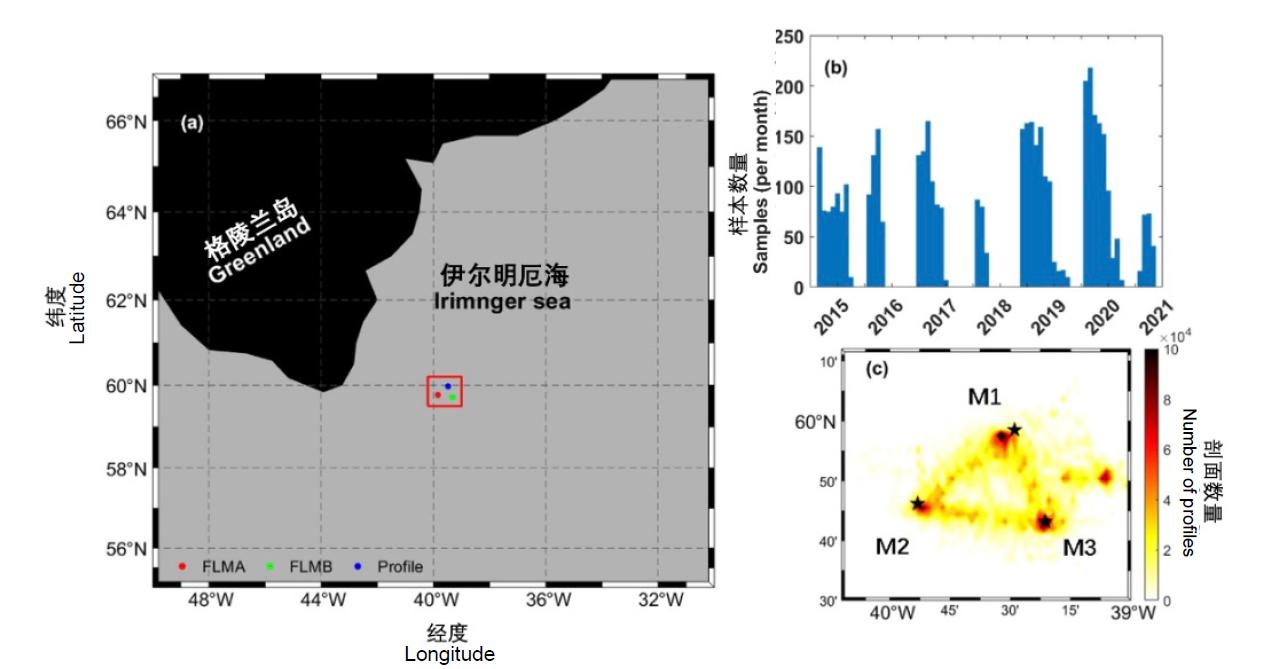
\includegraphics[width=0.8\linewidth]{img/fig_1_1_study_area.jpg}
    \figurecaption{(a) OOI项目位置,红框表示研究区域,彩色的点表示系泊。(b) 抽样概况的时间分布。(c) 采样点的空间分布,黑色的星星表示(a)中的系泊浮标}{(a) Position of OOI program, red box represents the study region, colored points indicate moorings. (b) Time distribution of sampling profiles. (c) Spatial distribution of sampling points, the blacks stars indicate the moorings in (a)}
    \label{fig:enter-label}
\end{figure}

\begin{figure}[htbp]
    \centering
    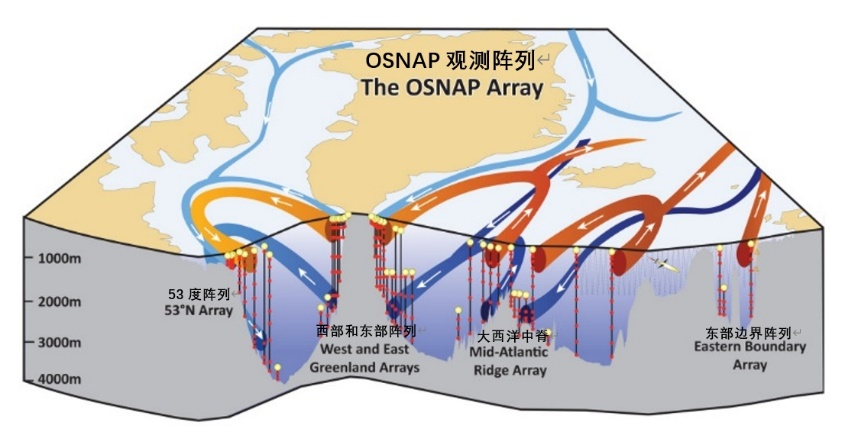
\includegraphics[width=0.5\linewidth]{img/fig_1_2_OSNAP.jpg}
    \figurecaption{北大西洋副极地翻转环流观测项目(OSNAP)阵列观测点(黄色点)空间分布}{Spatial distributions of OSNAP array observations (yellow dots)}
    \label{fig:enter-label}
\end{figure}

{\color{red}``图序采用阿拉伯数字分章编号,如第3章第2个图的图序为“图3-2”;英文标题,以Fig. 1-1编号。全文编号方式应统一。"}

\section{本章小结}
\ensection{Summary of this chapter}

前文中,我们回顾了中尺度涡旋、亚中尺度运动和近惯性内波以及它们之间的相互作用关系,然而前任工作对上述物理过程的研究往往是分散的,主要集中于讨论两两之间的相互作用,且具有时间或空间上的依赖性的,导致不同物理过程之间的相互作用的研究工作很难整合到一起$\cdots\cdots$
\chapter{数据与主要方法}
\enchapter{Data and methods}

\section{数据}
\ensection{Datasets}

\subsection{船载ADCP数据}
\ensubsection{ADCP data}

本文使用了Nuka Arctica邮轮船载声学多普勒流速剖面仪(Acoustic Doppler Current Profiler, ADCP)测量的上层海洋高空间分辨率流速资料。

XXXXXXXX。

\section{分析方法}
\ensection{Analysis methods}

\subsection{Wave-Vortex分解}
\ensubsection{Wave-Vortex}

本文使用了Wave-Vortex分解方法对船载ADCP测量结果进行了分析,参照Bühler提出的波-涡分解方法,采用一维动能谱的Wave-Vortex动能谱分解办法。这种方法能够解决由空间尺度上波动和涡动的尺度重叠导致二者在空间谱上信号混杂的问题。但分解方法和其他湍流分析一样有严格的假设:(1)数据测量稳定均匀,(2)各向同性,(3)数据在观测空间尺度上具有周期性。

首先,我们将跨航迹流速和沿航迹动能谱通过Helmholtz分解,转化为旋转和辐散两部分,将其写成谱函数的形式:

\begin{equation}
k\frac{\mathrm{d}\widehat{F}^{\phi}}{\mathrm{d}k}-\mathrm{d}\widehat{F}^{\psi}=-\frac{\widehat{C}^{v}}{2}
\end{equation}

\begin{equation}
k\frac{\mathrm{d}\widehat{F}^{\psi}}{\mathrm{d}k}-\mathrm{d}\widehat{F}^{\phi}=-\frac{\widehat{C}^{u}}{2}
\end{equation}

{\color{red}``对于别人论文里的公式,可以截图粘贴到豆包里转化为 latex 代码,效率非常高"}

式中,($\widehat{F}{\phi}$, $\widehat{F}{\psi}$)为计算过程谱函数,($\widehat{C}^{u}$, $\widehat{C}^{v}$)分别为沿航迹函数和跨航迹函数,$k$为水平波数……




\chapter{引用文献}
\section{文献引用测试章节}
学校前身是创办于1924年的私立青岛大学\cite{lamport94}。1930年,在省立山东大学和私立青岛大学的基础上成立国立青岛大学。后历经国立山东大学、山东大学时期\cite{dwx},1958年山东大学主体迁往济南,以留青的海洋系、水产系、地质系、生物系等为基础,于1959年3月成立山东海洋学院。1960年被确定为全国13所重点综合性大学之一。1988年更名为青岛海洋大学。2002年更名为中国海洋大学。

Lorem ipsum dolor sit amet\cite{xd}, consectetur adipiscing elit, sed do eiusmod tempor
incididunt ut labore et dolore magna aliqua.
Ut enim ad minim veniam, quis nostrud exercitation ullamco laboris nisi ut
aliquip ex ea commodo consequat.
Duis aute irure dolor in reprehenderit in voluptate velit esse cillum dolore eu
fugiat nulla pariatur.
Excepteur sint occaecat cupidatat non proident, sunt in culpa qui officia
deserunt mollit anim id est laborum.


\chapter{引用文献演示}

\section{文献引用测试章节}

学校前身是创办于1924年的私立青岛大学\cite{wc24arfm}。1930年,在省立山东大学和私立青岛大学的基础上成立国立青岛大学。后历经国立山东大学、山东大学时期\cite{zz19nc},1958年山东大学主体迁往济南\cite{lj15hyxb},以留青的海洋系、水产系、地质系、生物系等为基础,于1959年3月成立山东海洋学院。1960年被确定为全国13所重点综合性大学之一。1988年更名为青岛海洋大学。2002年更名为中国海洋大学。

Lorem ipsum dolor sit amet\cite{kj25tvcg}, consectetur adipiscing elit, sed do eiusmod tempor incididunt ut labore et dolore magna aliqua\cite{lcy24tgrs}. Ut enim ad minim veniam, quis nostrud exercitation ullamco laboris nisi ut aliquip ex ea commodo consequat. Duis aute irure dolor in reprehenderit in voluptate velit esse cillum dolore eu fugiat nulla pariatur. Excepteur sint occaecat cupidatat non proident, sunt in culpa qui officia deserunt mollit anim id est laborum.
\chapter{结论与展望}

\section{结论}

北大西洋作为大西洋深层水的发源地,对全球气候变化有着重要影响[6]。本文围绕中尺度过程、亚中尺度过程和近惯性内波之间的能量交换过程展开了一系列研究。首先,利用船载ADCP对Iceland Basin 和Irminger Sea的中尺度-亚中尺度运动和海洋内波的动能波数谱进行研究。讨论了中尺度过程、亚中尺度过程之间的转换尺度影响因素,季节变化特征和深度依赖性。其次,本文结合平衡流波数谱和三阶结构函数深入分析了两个海盆的能量串级和能量注入问题。进一步,由于亚中尺度能量注入问题和海洋斜压不稳定密切相关,本文利用Irminger Sea 阵列观测周围的水下滑翔机数据分析了亚中尺度锋面的季节特征和变化规律,并进一步分析了海洋多种类型的不稳定。最后,利用Iceland Basin 和Irminger Sea锚定浮标观测序列分析了中尺度、亚中尺度和近惯性内波之间的能量交换特征。本文得到以下结论:

北大西洋中尺度-亚中尺度运动与海洋内波,存在明显的季节变化特征。中尺度—亚中尺度运动在冬季动能谱斜率更接近于-5/3,在其他季节接近-3,说明除冬季外,上层海洋主要由准地转湍流过程调控。海洋内波在冬季最强,在夏季最弱。二者之间的转换尺度在夏季最小为28千米,在冬季海洋内波在各个尺度上超过中尺度-亚中尺度运动。这种转换尺度的巨大变化主要由海洋内波过程引……  

\section{展望}

北大西洋作为大西洋深层水的发源地,对全球气候变化有着重要影响[6]。本文围绕中尺度过程、亚中尺度过程和近惯性内波之间的能量交换过程展开了一系列研究。首先,利用船载ADCP对Iceland Basin 和Irminger Sea的中尺度-亚中尺度运动和海洋内波的动能波数谱进行研究。讨论了中尺度过程、亚中尺度过程之间的转换尺度影响因素,季节变化特征和深度依赖性。其次,本文结合平衡流波数谱和三阶结构函数深入分析了两个海盆的能量串级和能量注入问题。进一步,由于亚中尺度能量注入问题和海洋斜压不稳定密切相关,本文利用Irminger Sea 阵列观测周围的水下滑翔机数据分析了亚中尺度锋面的季节特征和变化规律,并进一步分析了海洋多种类型的不稳定。最后,利用Iceland Basin 和Irminger Sea锚定浮标观测序列分析了中尺度、亚中尺度和近惯性内波之间的能量交换特征。本文得到以下结论:

北大西洋中尺度-亚中尺度运动与海洋内波,存在明显的季节变化特征。中尺度—亚中尺度运动在冬季动能谱斜率更接近于-5/3,在其他季节接近-3,说明除冬季外,上层海洋主要由准地转湍流过程调控。海洋内波在冬季最强,在夏季最弱。二者之间的转换尺度在夏季最小为28千米,在冬季海洋内波在各个尺度上超过中尺度-亚中尺度运动。这种转换尺度的巨大变化主要由海洋内波过程引……  

% 参考文献
\phantomsection\addengcontent{chapter}{References}
\bibliographystyle{oucauthoryear}
\bibliography{cite}

% 学术成果
\phantomsection\addengcontent{chapter}{Published papers and research results}
\begin{achievement}

\par \vskip10pt
{\fontsize{14pt}{21pt}\selectfont\heiti 一、发表的学术论文}
\par \vskip10pt

学术论文1

学术论文2

\par \vskip10pt
{\fontsize{14pt}{21pt}\selectfont\heiti 二、申请及已获得的专利}
\par \vskip10pt

专利1

专利2


\par \vskip10pt
{\fontsize{14pt}{21pt}\selectfont\heiti 三、参与的科研项目及获奖情况}
\par \vskip10pt

获奖1

获奖2


\end{achievement}

% 致谢
\phantomsection\addengcontent{chapter}{Acknowledgements}
\begin{ackonwlegmentback}

致谢中主要感谢导师和对论文工作有直接贡献或帮助的人士和单位。

一般致谢的内容有:

(1)对国家科学基金、资助研究工作的奖学金基金、合同单位、资助或支持的企业、组织或个人;

(2)对协助完成研究工作和提供便利条件的组织或个人;

(3)对在研究工作中提出建议和提供帮助的人;

(4)对给予转载和引用权的资料、图片、文献、研究思想和设想的所有者;

(5)对其他应感谢的组织和个人;

(6)致谢言语应谦虚诚恳,实事求是,建议字数不超过1000字。

\end{ackonwlegmentback}

% 作者简介
\phantomsection\addengcontent{chapter}{Resume}
\begin{profile}

主要包括姓名、性别、民族、出生年月、出生地;简要学习、工作经历;以及攻读学位期间获得的其他奖励(除攻读学位期间取得的与学位论文相关的成果之外)。个人简历一般应包含从本科起的教育经历和工作经历。示例:

××××年××月××日出生于××××。

××××年××月考入××大学××院(系)××专业,××××年××月本科毕业并获得××学学士学位。

××××年××月——××××年××月,在××大学××院(系)××学科学习并获得××学硕士学位。

××××年××月——××××年××月,在××大学××院(系)××学科攻读博士学位。

获奖情况:如获三好学生、优秀团干部、×奖学金等(不含科研学术获奖)。

工作经历:

\end{profile}


\end{document}
